\documentclass[conference]{IEEEtran}
\usepackage{cite}
\usepackage{amsmath,amssymb,amsfonts}
\usepackage{algorithmic}
\usepackage{graphicx}
\usepackage{textcomp}
\usepackage{xcolor}
\def\BibTeX{{\rm B\kern-.05em{\sc i\kern-.025em b}\kern-.08em
    T\kern-.1667em\lower.7ex\hbox{E}\kern-.125emX}}
\begin{document}
\selectlanguage{dutch}

\title{Digitale kunstcollecties ontdekken door middel van Link-Traversal–based Query Processing}

\author{\IEEEauthorblockN{Martijn Bogaert}
\IEEEauthorblockA{
\textit{Universiteit Gent}\\
Gent, België \\
martijn.bogaert@ugent.be}}

\maketitle

\begin{abstract}
Deze masterproef onderzoekt het verkennen van digitale kunstcollecties via Link-Traversal-based Querying, met de focus op de \textit{Collectie van de Gentenaar}. Het Comunica-platform speelt een sleutelrol bij het benutten van waardevolle data in RDF-formaat, hoewel sommige links uitdagingen met RDF-compatibiliteit opleveren. Twee webapplicatie-ideeën worden voorgesteld om zowel gebruikers zonder technische achtergrond als professionals te helpen bij het verkennen van de CoGent-collectie. Het einddoel is om ontdekte data te koppelen aan IIIF Manifests voor visualisatie en zo de toegankelijkheid van kunstcollecties te vergroten.
\end{abstract}

\begin{IEEEkeywords}
Linked Data, Link Traversal, LTQP, CoGent, IIIF
\end{IEEEkeywords}

\section*{Inleiding}
Digitale kunstcollecties belichamen menselijke creativiteit en culturele ontwikkeling. Door technologische vooruitgang zijn deze verzamelingen gedigitaliseerd, waardoor ze wereldwijd toegankelijk zijn en diepgaand kunnen worden verkend. Toch brengt het navigeren en bevragen van deze gegevens uitdagingen met zich mee, vooral voor niet-technische professionals en kunstliefhebbers. Deze beperking belemmert hun vermogen om inzichten te verwerven en volledig op te gaan in de wereld van digitale kunst.

De culturele data van de Collectie van de Gentenaar (CoGent) worden gepubliceerd volgens de principes van Linked Data, waardoor ze stevig verankerd zijn in het semantische web. Maar om het volledige potentieel van deze uitgebreide gegevens te benutten, is Link-Traversal–based Query Processing (LTQP) vereist. LTQP stelt gebruikers namelijk in staat om buiten de grenzen van de dataset te treden, waardoor lagen van kennis en verbindingen kunnen worden blootgelegd die anders verborgen zouden blijven.

Het onderzoek ontleedt het \textit{ontdekken} van de CoGent-gegevens in drie fundamentele onderdelen: het opstellen van queries, het uitvoeren van queries met behulp van linktraversal - de van het onderzoek - en het verwerken van queryresultaten, met name de visualisatie en opslag ervan. Deze opgedeelde aanpak legt de basis voor een diepgaandere verkenning van de CoGent-data en mogelijks digitale kunstcollecties in het algemeen.

\section{Gerelateerd werk}

\subsection{Collectie van de Gentenaar}
Dit onderzoek richt zich voornamelijk op de gegevens van de \textit{Collectie van de Gentenaar} (CoGent), of \textit{Collections of Ghent} (CoGhent) in het Engels. CoGent is een samenwerkingsverband tussen de stad Gent, Design Museum Gent, Digipolis en andere lokale organisaties. Samen hebben ze als doel het cultureel erfgoed van de stad te verzamelen en te digitaliseren in een centrale collectie, waarbij bewoners van Gent worden aangemoedigd om hun eigen erfgoedverhalen en objecten ook toe te voegen. Hoewel de CoGent-partnerschap in juni 2023 werd beëindigd, blijft de infrastructuur behouden. \cite{leemputten2022gent} \cite{schouppe2022gent}

De gegevens van de deelnemende culturele instellingen, namelijk Design Museum Gent (DMG), Huis van Alijn (HVA), Industriemuseum, STAM en Archief Gent, worden beheerd in Linked Data Event Streams (LDES). LDES'en zijn collecties onveranderlijke objecten die voorgesteld worden door RDF triples. Dat de objecten onveranderlijk zijn, betekent dat zodra een object wordt toegevoegd, het ongewijzigd blijft. Nieuwe versies van objecten worden geïntroduceerd in plaats van bestaande objecten te updaten. \cite{floreverk2022coghent} \cite{colpaert2023ldes}

De LDES'en van CoGent in het bijzonder, bevatten \textit{Mensgemaakte Objecten}, of \textit{Human-Made Objects} in het Engels. Deze vertegenwoordigen zowel tastbare als ontastbare items die door mensen zijn gemaakt of beïnvloed, variërend van kunstwerken en boeken tot tradities en ambachten. Het \textit{Open Standaarden voor Linkende Organisaties}-initiatief (OSLO) speelt een cruciale rol in de standaardisatie deze Mensgemaakte Objecten. Mensgemaakte Objecten zijn ook volledig in lijn met internationale normen met het oog op semantische interoperabiliteit binnen het domein van cultureel erfgoed. \cite{van2022publishing} \cite{vanderperren2021oslo}

\subsection{International Image Interoperability Framework}
Elk Mensgemaakt Object in de collecties van CoGent bevat, naast zijn beschrijvende data, een link naar een IIIF Manifest. Deze manifests zijn gestructureerde RDF-bronnen die specifieke informatie over een object groeperen, variërend van details zoals dimensies en notities tot auteursrechtelijke informatie. Het International Image Interoperability Framework (IIIF) legt via haar Presentation en Image API's vast hoe deze manifests opgebouwd dienen te worden. In het geval van CoGent manifests, is die opbouw zeer eenvoudig: elk manifest bevat één sequence, die op haar beurt één canvas bevat, die op haar beurt dan weer één annotation met de afbeeldingslink en -metadata bevat. \cite{appleby2017presentation} \cite{emanuel2018stitching} \cite{floreverk2022coghent}

Naast de opslag van deze gegevens, zijn IIIF Manifests vooral bijzonder handig om culturele data te visualiseren. Er bestaan reeds meerdere IIIF Viewers die dit bewerkstelligen. Voor een gegeven manifest bieden deze viewers een gestandaardiseerde weergave van de data die erin aanwezig zijn. \cite{snydman2015international}

\subsection{Link-Traversal-based Query Processing}
Dat de CoGhent-collecties deel uitmaken van het Linked Data web, maakt dat ze in principe veel meer knowledge kunnen voortbrengen dan wanneer de enkel de CoGhent-data op zich bevraagd wordt. Deze \textit{externe} data proberen te bereiken met één SPARQL query, kan echter enkel wanneer de uitvoerende query engine van resource naar resource kan \textit{springen}. Link Traversal-based Query Processing (LTQP) maakt dit praktisch mogelijk door dynamisch links tussen documenten te volgen. \cite{taelman2023ltqp}

Echter, zonder beperkingen op te leggen aan de te volgen links, is LTQP onpraktisch. Daarom introduceerde O. Hartig \cite{hartig2012foundations} drie \textit{reachability criteria}: 
\begin{itemize}
    \item \textit{cAll} volgt alle links zonder beperking.
    \item \textit{cNone} volgt geen enkele link.
    \item \textit{cMatch} volgt alleen links die deel uitmaken van quads die overeenkomen met een quad pattern uit de query.
\end{itemize}

Dankzij haar modulariteit en aanpasbaarheid, kunnen de bovengenoemde en andere capaciteiten aan een Comunica engine gegeven worden, waardoor LTQP in de praktijk mogelijk wordt. \cite{taelman2018comunica} \cite{taelman2019lt}

\section{CoGent data en link traversal}

\subsection{CoGent-bronnen}
CoGent biedt voor elke deelnemende culturele instelling een aparte LDES aan. Dit kan handig zijn om bij aanvang van het querying proces een onderscheid te maken tussen verschillende collecties. In theorie is het ook zo dat de volgorde waarin de URI's van deze LDES'en als datasources aan een Comunica link traversal engine meegeven worden, bepaalt welke collectie eerst bevraagd wordt en uiteindelijk de eerste resultaten terug zal geven. In de praktijk ligt dat echter anders. Wanneer een link traversal engine verschillende HTTP requests uitvoert, is het immers niet op voorhand vast te leggen in welke volgorde de overeenkomstige HTTP responses de engine weer zullen bereiken. Of nog: hoe verder de engine in haar \textit{link traversal proces} gevordered is, hoe meer \textit{willekeur} vastgesteld kan worden.

Dit maakt niet alleen dat de volgorde waarin LDES'en opgegeven worden, in principe weinig uitmaakt, maar ook dat de Mensgemaakte Objecten die in één bepaalde LDES voorkomen, niet per se in diezelfde volgorde teruggegeven zullen worden. Naast de vele voordelen, moet men er zich dus goed bewust van zijn dat LTQP ook duidelijk zijn nadelen heeft. Echter, aangezien de CoGhent-collecties in principe LDES'en zijn, zou er sowieso nooit van uit gegaan mogen worden dat dezelfde query op verschillende momenten dezelfde resultaten terug zou geven. LDES'en worden immers precies gekenmerkt door hun grote variabiliteit.

\subsection{Comunica link traversal engine configuratie}
Comunica biedt reeds meerdere modules en configuraties aan die LTQP op allerhande verschillende manieren mogelijk moeten maken. Bij het opstellen van een configuratie voor een link traversal engine, moeten in eerste instantie in principe telkens dezelfde actoren aan bod. Zij staan in voor de basisfunctionaliteit van elke link traversal engine. Deze basisconfiguratie wordt aangeboden in een apart configuratiebestand, \textit{config-base.json} en moet dus zeker opgenomen worden in de uiteindelijke configuratie die het meest geschikt geacht zal worden voor het uitvoeren van LTQP op de CoGhent-LDES'en.

Een essentiële keuze die wel voor elke configuratie gemaakt moet worden, is de selectie van een link extractor. Dergelijk type actor bepaalt immers voor elk document dat binnenkomt, welke links daaruit toegevoegd dienen te worden aan de link queue en dus bezocht moeten worden. De meest voor de hand liggende keuzes zijn in dat opzicht de \textit{All Extract Links Actor} en \textit{Quad Pattern Query Extract Links Actor}. In principe zijn zij implementaties van de respectievelijke \textit{cAll} en \textit{cMatch} reachability criteria. Het hoeft echter niet te verbazen dat de \textit{All Extract Links Actor} zonder bijkomende begrenzingen in de praktijk geen valabele keuze is. Een engine die zomaar elke link volgt, kan immers tot in het oneindige links blijven volgen wiens documenten uiteindelijk toch niet de informatie bevatten waarnaar de query op zoek is. De \textit{Quad Pattern Query Extract Links Actor} is daarentegen wel een valabele optie, zeker vanuit de optiek van deze research. De research gaat immers op zoek naar datapunten die specifiek \textit{toebehoren} aan Mensgemaakte Objecten. Het is met andere woorden vanop voorhand geweten welke \textit{paden} vanuit een Mensgemaakt Object naar de datapunten in kwestie gevolgd dienen te worden. Aangezien dit weergegeven wordt door de query, zal een \textit{Quad Pattern Query Extract Links Actor} op zijn minst de \textit{juiste} links volgen, maar bovenal een potentieel groot aantal \textit{verkeerde} links negeren.

Naast deze \textit{standaard} link extractors, biedt Comunica nog enkele bijkomende aan. Eén daarvan, de \textit{Predicates Extract Links Actor} is voor deze research in het bijzonder een erg interessante. De \textit{Predicates Extract Links Actor} gaat namelijk nog gerichter op zoek naar links door uitsluitend links die als object in een quad voorkomen, te beschouwen, maar pas aan de link queue toe te voegen wanneer hun predicate overeenkomt met een van de regexen die in de actor configuratie bepaald zijn. Aangezien de op voorhand bekende \textit{paden} van Mensgemaakte Objecten naar gezochte datapunten in principe uitsluitend bepaald worden door sequenties van predicaten, garandeert deze link extractor dan ook de snelste uitvoeringstijd. Het grote nadeel aan deze actor is echter dat voor elke nieuwe query een nieuwe engine aangemaakt moet worden, waardoor het gebruik ervan minder toegankelijk is. Toch hoeft dit in het kader van dit onderzoek geen probleem te vormen. De research culmineert immers sowieso in enkele gebruikersgerichte applicaties, die naast hun hoofdfunctionaliteiten evengoed ook deze technische complexiteit van gebruikers kunnen \textit{wegabstraheren}.

Door het expliciet instellen van predicaten, steekt een nieuwe uitdaging de kop op: de links die voor een gegeven LDES-pagina naar de voorgaande en/of volgende pagina verwijzen, worden niet meer gevolgd, waardoor de engine per opgegeven LDES slechts één pagina kan beschouwen. De verschillende predicaten die naar deze links lopen, zouden in principe aan de predicatenlijst toegevoegd kunnen worden, ware het niet dat er reeds een link extractor bestaat die nadrukkelijk op zoek gaat naar \textit{TREE-specifieke} links. Aangezien de LDES-specificatie gebouwd is op de TREE-specificatie, is het dan ook aangewezen de huidige configuratie uit te breiden met deze \textit{Extract Links Tree Actor} en zo de volledige collecties bij het queryproces te betrekken. \cite{colpaert2023tree}

\subsection{Te volgen links}
Met de beschreven configuratie, zou de volgende stap het opstellen van queries moeten zijn. Alleen blijkt het semantische web in de praktijk minder \textit{querybaar} te zijn als verhoopt. Een groot probleem is namelijk dat bepaalde resources niet volledig volgens de richtlijnen worden gehost. Ook enkele van de types resources waarnaar CoGent Mensgemaakte Objecten refereren, lijden aan dergelijk euvel, waardoor het bijzonder moeilijk en soms zelfs onmogelijk wordt om hen te betrekken tijden het link traversalproces.

\subsubsection{CoGhent IIIF Manifests}
Beginnen met het goede nieuws: de IIIF Manifests die de visuele component van Human-Made Objects beschrijven, zijn zonder meer bereikbaar en interpreteerbaar voor een link traversal engine. De digitale afbeelding van een Human-Made Object kan met andere woorden probleemloos opgehaald worden naast eventuele andere (tekstuele) data.

\subsubsection{Wikidata}
Ook met Wikidata resources heeft een link traversal engine in principe geen probleem. Toch moet hierbij een opmerking gemaakt worden. Wikidata voorziet voor elke resource en property immers twee URIs. De \textit{standaard} URIs die Wikidata zeer expliciet \textit{adverteert}, zijn het soort URIs waar andere bronnen - ook de CoGhent LDESs - doorgaans naar verwijzen. Echter, dit zijn niet de URIs die Wikidata \textit{achter de schermen} gebruikt om haar RDF-data mee te beschrijven. Voor een link traversal engine is dit geen probleem, die wordt immers automatisch \textit{geredirectet} naar de juist RDF-URI, maar gebruikers moeten wel op hun hoede zijn. Wanneer in een query een Wikidata-URI dient voor te komen moet namelijk expliciet gebruik gemaakt worden van de RDF-specifieke variant. Dit is belangrijk voor het soort queries centraal in deze research, aangezien deze typisch datapunten proberen te bereiken door middel van \textit{paden} die bestaan uit één of meerdere expliciet bepaalde predicaat-URIs.

\subsubsection{Stad Gent data}
Wanneer een Comunica link traversal engine een Stad Gent resource probeert te bevragen, zal dit helaas steeds mislukken. Dit valt toe te wijzen aan een configuratiefout van de Stad Gent server. Deze zal immers steeds met een \textit{Content-Type} van \textit{application/json} reageren op de \textit{Accept} header die Comunica voor haar HTTP requests instelt, terwijl de content wel degelijk een volwaardig JSON-LD-document is. Nochtans zou dit in principe geen probleem mogen zijn, ware het niet dat de server bij haar \textit{JSON-bestand} geen context link header meegeeft, terwijl Comunica dit (terecht) verwacht. Totdat de Stad Gent server correct geconfigureerd is - niet het geval bij publicatie van de research - kunnen hun resources dan ook niet bereikt worden door een Comunica link traversal engine.

\subsubsection{Getty Vocabularies}
Ook de Getty Vocabularies server lijkt aan een gelijkaardige configuratiefout te lijden. Ook die geeft op basis van Comunica's \textit{Accept} header JSON content terug zonder context link header. Gelukkig kan voor de Getty Vocabularies resources een omweg genomen worden: wanneer expliciet de \textit{.json-ld}-extensie aan hun URIs toegevoegd wordt, reageert de server immers met een \textit{Content-Type} van \textit{application/ld+json}. Om een Comunica link traversal engine van deze capaciteit te voorzien, moet echter een custom actor aangemaakt worden die elke link uit een gegeven document overloopt en er zo nodig de extensie aan toevoegt. Dankzij deze tussenkomst is het mogelijk Getty Vocabularies resources in het link traversalproces te betrekken, maar het is duidelijk dat deze oplossing niet optimaal is.

\section{Tools voor de constructie van queries}
Een belangrijk doel van de research is om gebruikers zonder technische achtergrond toch de mogelijkheid te geven de CoGent-collecties, in combinatie met alle data waarnaar ze verwijzen, te ontdekken. Zij moeten met andere woorden in staat gesteld worden de nodige queries - zij het eenvoudige - daarvoor op te stellen. In het licht daarvan introduceert de research dan ook twee gebruiksvriendelijke tools om in dit proces te helpen. Beide tools steunen echter op hetzelfde idee: op basis van gegeven input een query opstellen. Daarom maken beiden gebruik van een andere, meer \textit{low-level} applicatie.

\subsection{Queryconstructie door middel van predicaatsequenties}
SPARQL queries kunnen zeer complexe vormen aannemen, maar in deze research wordt gefocust op het eerder eenvoudige soort queries dat voor een bepaald type resources - Mensgemaakte Objecten - één of meerdere kenmerkende \textit{properties} ophaalt door \textit{paden} aan predicaten - \textit{predicate sequences} - in de query te stipuleren. Deze specifieke manier van werken staat toe een eenvoudige applicatie te bouwen die een query kan genereren op basis van een op voorhand bepaalde reeks - kan er ook één zijn - \textit{properties} die dan weer elk een reeks predicaten specificeert. Daarnaast kan elke \textit{property} ook als \textit{optioneel} bestempeld en/of gefilterd worden.

\subsection{Gebruikersgerichte applicaties}
Bijkomend worden twee andere applicaties geïntroduceerd. Hun voornaamste doel is het aanbieden van een gebruiksvriendelijke interface om queries op te bouwen, terwijl ze voor het effectieve query-generatieproces op de voorgaande tool kunnen rekenen.

De eerste applicatie is voor de minst technische gebruikers bedoeld en is dan ook de meest eenvoudige: gebruikers krijgen een overzicht van vooraf bepaalde \textit{properties} te zien en kunnen hieruit een keuze maken. Daarnaast krijgen ze onder andere ook de mogelijkheid filters te specificeren. Dankzij een eenvoudige \textit{klik op de knop} krijgen ze ten slotte de overeenkomstige query te zien.

De tweede applicatie is wat uitdagender in gebruik, maar beperkt gebruikers in hun keuze niet uitsluitend tot de \textit{properties} die door anderen \textit{voorgekauwd} zijn. Gebruikers worden geacht eigenhandig een resource op te geven, vanwaaruit ze een boom aan predicaten en andere resources kunnen doen vertakken. Dit geeft hen niet alleen een inkijk in het soort data waartoe het opgegeven type resource toegang verleent, maar biedt ook de mogelijkheid uit de bekomen boom resources als \textit{properties} te selecteren en er onder andere filters voor in te stellen. Opnieuw krijgen gebruikers dankzij een eenvoudige \textit{klik op de knop} ten slotte de overeenkomstige query te zien.

\section{Queryresultaten verwerken}
TODO

\subsection{Queryresultaten visualiseren}
TODO

\subsection{Queryresultaten opslaan}
TODO

\section*{Conclusie}
TODO

\section*{Dankwoord}
TODO

\bibliographystyle{IEEEtran}
\bibliography{references}

\end{document}


% \begin{table}[htbp]
% \caption{Table Type Styles}
% \begin{center}
% \begin{tabular}{|c|c|c|c|}
% \hline
% \textbf{Table}&\multicolumn{3}{|c|}{\textbf{Table Column Head}} \\
% \cline{2-4} 
% \textbf{Head} & \textbf{\textit{Table column subhead}}& \textbf{\textit{Subhead}}& \textbf{\textit{Subhead}} \\
% \hline
% copy& More table copy$^{\mathrm{a}}$& &  \\
% \hline
% \multicolumn{4}{l}{$^{\mathrm{a}}$Sample of a Table footnote.}
% \end{tabular}
% \label{tab1}
% \end{center}
% \end{table}

% \begin{figure}[htbp]
% \centerline{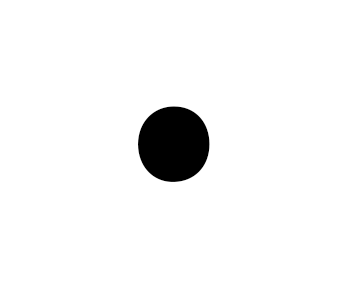
\includegraphics{fig1.png}}
% \caption{Example of a figure caption.}
% \label{fig}
% \end{figure}